\documentclass[11pt,a4paper]{report}
\usepackage[textwidth=37em,vmargin=30mm]{geometry}
\usepackage{calc,xunicode,amsmath,amssymb,paralist,enumitem,tabu,booktabs,datetime2,xeCJK,xeCJKfntef,listings}
\usepackage{tocloft,fancyhdr,tcolorbox,xcolor,graphicx,eso-pic,xltxtra,xelatexemoji}

\newcommand{\envyear}[0]{2025}
\newcommand{\envdatestr}[0]{2025-09-11}
\newcommand{\envfinaldir}[0]{webdb/2025/20250911/final}

\usepackage[hidelinks]{hyperref}
\hypersetup{
    colorlinks=false,
    pdfpagemode=FullScreen,
    pdftitle={Web Digest - \envdatestr}
}

\setlength{\cftbeforechapskip}{10pt}
\renewcommand{\cftchapfont}{\rmfamily\bfseries\large\raggedright}
\setlength{\cftbeforesecskip}{2pt}
\renewcommand{\cftsecfont}{\sffamily\small\raggedright}

\setdefaultleftmargin{2em}{2em}{1em}{1em}{1em}{1em}

\usepackage{xeCJK,xeCJKfntef}
\xeCJKsetup{PunctStyle=plain,RubberPunctSkip=false,CJKglue=\strut\hskip 0pt plus 0.1em minus 0.05em,CJKecglue=\strut\hskip 0.22em plus 0.2em}
\XeTeXlinebreaklocale "zh"
\XeTeXlinebreakskip = 0pt


\setmainfont{Brygada 1918}
\setromanfont{Brygada 1918}
\setsansfont{IBM Plex Sans}
\setmonofont{JetBrains Mono NL}
\setCJKmainfont{Noto Serif CJK SC}
\setCJKromanfont{Noto Serif CJK SC}
\setCJKsansfont{Noto Sans CJK SC}
\setCJKmonofont{Noto Sans CJK SC}

\setlength{\parindent}{0pt}
\setlength{\parskip}{8pt}
\linespread{1.15}

\lstset{
	basicstyle=\ttfamily\footnotesize,
	numbersep=5pt,
	backgroundcolor=\color{black!5},
	showspaces=false,
	showstringspaces=false,
	showtabs=false,
	tabsize=2,
	captionpos=b,
	breaklines=true,
	breakatwhitespace=true,
	breakautoindent=true,
	linewidth=\textwidth
}






\newcommand{\coverpic}[2]{
    % argv: itemurl, authorname
    Cover photo by #2~~(\href{#1}{#1})
}
\newcommand{\makeheader}[0]{
    \begin{titlepage}
        % \newgeometry{hmargin=15mm,tmargin=21mm,bmargin=12mm}
        \begin{center}
            
            \rmfamily\scshape
            \fontspec{BaskervilleF}
            \fontspec{Old Standard}
            \fontsize{59pt}{70pt}\selectfont
            WEB\hfill DIGEST
            
            \vfill
            % \vskip 30pt
            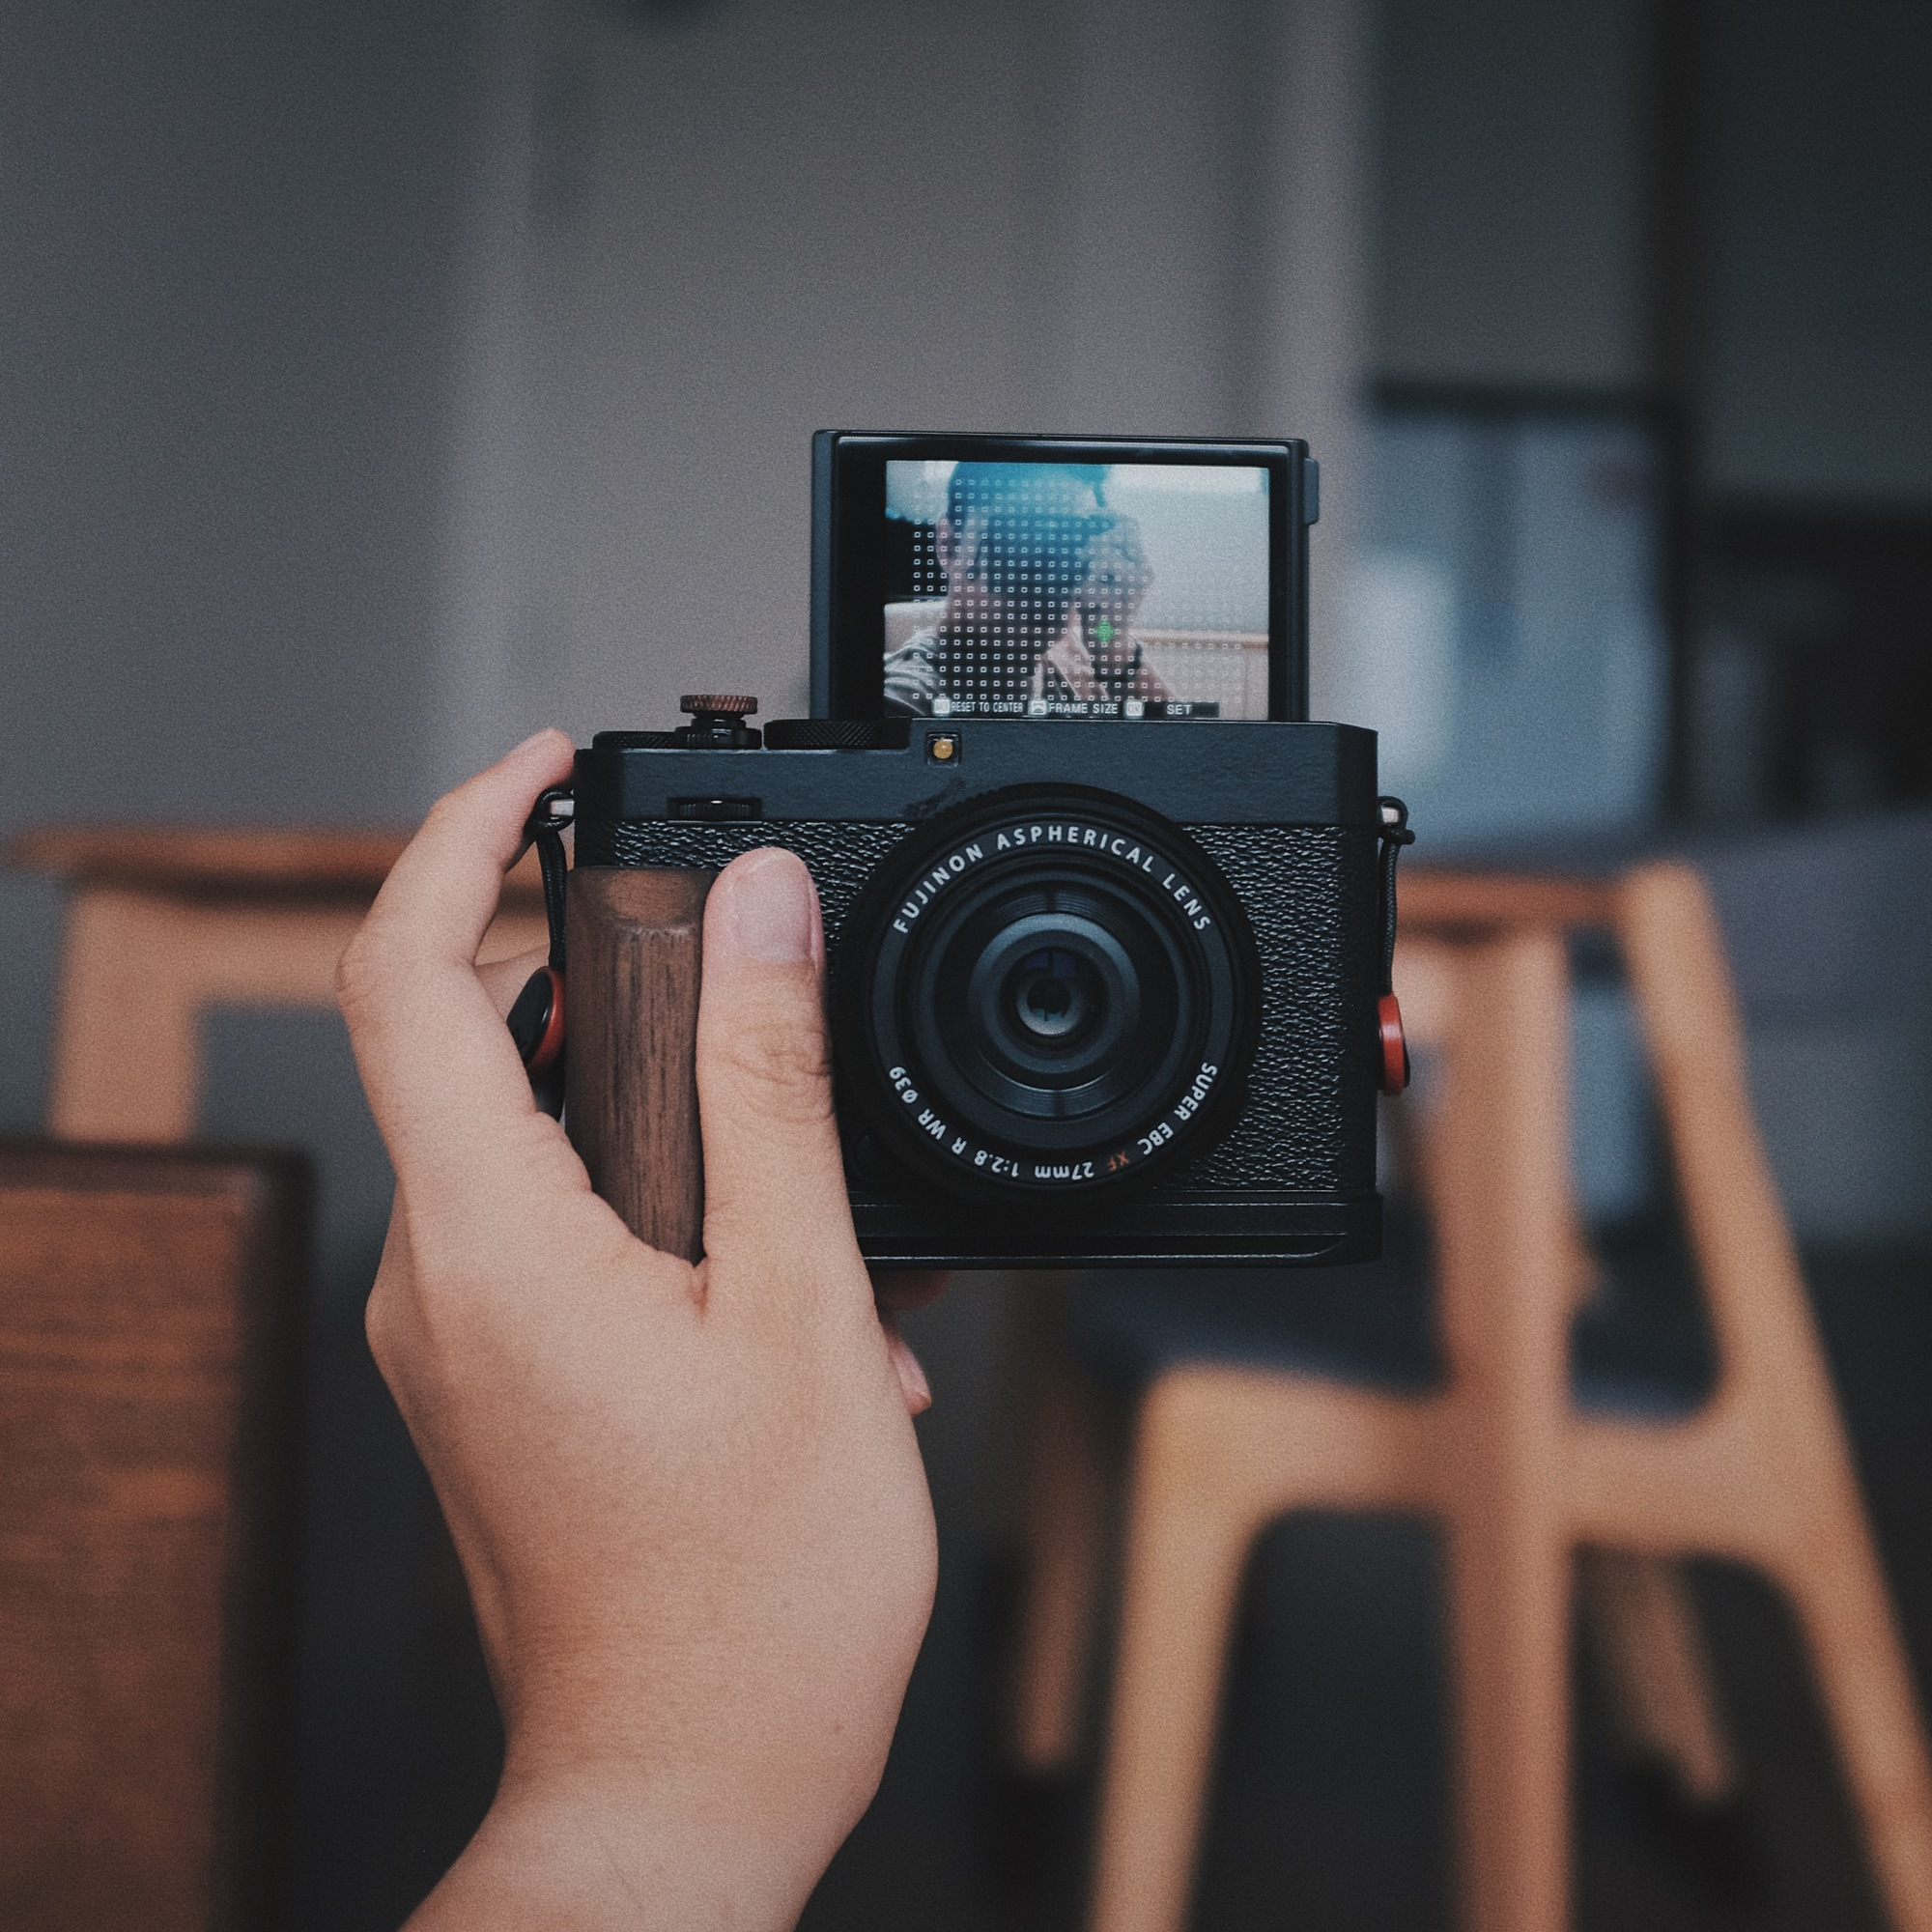
\includegraphics[width=\linewidth]{\envfinaldir/coverpic-prod.jpg}\par
            % \vskip 30pt
            \vfill

            \normalsize\rmfamily\scshape
            \copyright{} The Web Digest Project \hfill\large \envdatestr
        \end{center}
    \end{titlepage}
    % \restoregeometry
}
\newcommand{\simplehref}[1]{%
    \textcolor{blue!80!green}{\href{#1}{#1}}%
}
\renewcommand{\contentsname}{\center\Huge\sffamily\bfseries Contents\par\vskip 20pt}
\newcounter{ipartcounter}
\setcounter{ipartcounter}{0}
\newcommand{\ipart}[1]{
    % \vskip 20pt
    \clearpage
    \stepcounter{ipartcounter}
    \phantomsection
    \addcontentsline{toc}{chapter}{#1}
    % \begin{center}
    %     \Huge
    %     \sffamily\bfseries
    %     #1
    % \end{center}
    % \vskip 20pt plus 7pt
}
\newcounter{ichaptercounter}
\setcounter{ichaptercounter}{0}
\newcommand{\ichapter}[1]{
    % \vskip 20pt
    \clearpage
    \stepcounter{ichaptercounter}
    \phantomsection
    \addcontentsline{toc}{section}{\numberline{\arabic{ichaptercounter}}#1}
    \begin{center}
        \Huge
        \sffamily\bfseries
        #1
    \end{center}
    \vskip 20pt plus 7pt
}
\newcommand{\entrytitlefont}[1]{\subsection*{\raggedright\Large\sffamily\bfseries#1}}
\newcommand{\entryitemGeneric}[2]{
    % argv: title, url
    \parbox{\linewidth}{
        \entrytitlefont{#1}\par\vskip 5pt
        \footnotesize\ttfamily\mdseries
        \simplehref{#2}
    }\vskip 11pt plus 11pt minus 1pt
}
\newcommand{\entryitemGithub}[3]{
    % argv: title, url, desc
    \parbox{\linewidth}{
        \entrytitlefont{#1}\par\vskip 5pt
        \footnotesize\ttfamily\mdseries
        \simplehref{#2}\par\vskip 5pt
        \small\rmfamily\mdseries#3
    }\vskip 11pt plus 11pt minus 1pt
}
\newcommand{\entryitemAp}[3]{
    % argv: title, url, desc
    \parbox{\linewidth}{
        \entrytitlefont{#1}\par\vskip 5pt
        \footnotesize\ttfamily\mdseries
        \simplehref{#2}\par\vskip 5pt
        \small\rmfamily\mdseries#3
    }\vskip 11pt plus 11pt minus 1pt
}
\newcommand{\entryitemHackernews}[3]{
    % argv: title, hnurl, rawurl
    % \parbox{\linewidth}{
    %     \entrytitlefont{#1}\par\vskip 5pt
    %     \footnotesize\ttfamily\mdseries
    %     \simplehref{#3}\par
    %     \textcolor{black!50}{\href{#2}{#2}}
    % }\vskip 11pt plus 11pt minus 1pt
    \begin{minipage}{\linewidth}
            \entrytitlefont{#1}\par\vskip 5pt
            \footnotesize\ttfamily\mdseries
            \simplehref{#3}\par
            \textcolor{black!50}{\href{#2}{#2}}
    \end{minipage}\par\vskip 11pt plus 11pt minus 1pt
}







\begin{document}

\makeheader

\tableofcontents\clearpage




\ipart{Developers}
\ichapter{Hacker News}
\entryitemTwoLinks{KDE launches its own distribution}{https://news.ycombinator.com/item?id=45204393}{https://lwn.net/SubscriberLink/1037166/caa6979c16a99c9e/}

\entryitemTwoLinks{Charlie Kirk killed at event in Utah}{https://news.ycombinator.com/item?id=45202200}{https://www.nbcnews.com/news/us-news/live-blog/live-updates-shooting-charlie-kirk-event-utah-rcna230437}

\entryitemTwoLinks{Defeating Nondeterminism in LLM Inference}{https://news.ycombinator.com/item?id=45200925}{https://thinkingmachines.ai/blog/defeating-nondeterminism-in-llm-inference/}

\entryitemTwoLinks{'Block Everything' protests sweep across France, scores arrested}{https://news.ycombinator.com/item?id=45200357}{https://www.reuters.com/world/europe/block-everything-protests-sweep-across-france-scores-arrested-2025-09-10/}

\entryitemTwoLinks{API, Claude.ai, and Console services impacted [resolved]}{https://news.ycombinator.com/item?id=45200118}{https://status.anthropic.com/incidents/k6gkm2b8cjk9}

\entryitemTwoLinks{I didn't bring my son to a museum to look at screens}{https://news.ycombinator.com/item?id=45199931}{https://sethpurcell.com/writing/screens-in-museums/}

\entryitemTwoLinks{TikTok has turned culture into a feedback loop of impulse and machine learning}{https://news.ycombinator.com/item?id=45199760}{https://www.thenexus.media/tiktok-won-now-everything-is-60-seconds/}

\entryitemTwoLinks{ChatGPT Developer Mode: Full MCP client access}{https://news.ycombinator.com/item?id=45199713}{https://platform.openai.com/docs/guides/developer-mode}

\entryitemTwoLinks{Microsoft PowerToys}{https://news.ycombinator.com/item?id=45199191}{https://learn.microsoft.com/en-us/windows/powertoys/}

\entryitemTwoLinks{Zoox robotaxi launches in Las Vegas}{https://news.ycombinator.com/item?id=45199031}{https://zoox.com/journal/las-vegas}

\entryitemTwoLinks{Jiratui – A Textual UI for interacting with Atlassian Jira from your shell}{https://news.ycombinator.com/item?id=45198481}{https://jiratui.sh/}

\entryitemTwoLinks{We can't circumvent the work needed to train our minds}{https://news.ycombinator.com/item?id=45198420}{https://zettelkasten.de/posts/the-scam-called-you-dont-have-to-remember-anything/}

\entryitemTwoLinks{Performance Improvements in .NET 10}{https://news.ycombinator.com/item?id=45197608}{https://devblogs.microsoft.com/dotnet/performance-improvements-in-net-10/}

\entryitemTwoLinks{Guy running a Google rival from his laundry room}{https://news.ycombinator.com/item?id=45197187}{https://www.fastcompany.com/91396271/searcha-page-seekninja-diy-search-engines}

\entryitemTwoLinks{Kerberoasting}{https://news.ycombinator.com/item?id=45196437}{https://blog.cryptographyengineering.com/2025/09/10/kerberoasting/}

\entryitemTwoLinks{OrioleDB Patent: now freely available to the Postgres community}{https://news.ycombinator.com/item?id=45196173}{https://supabase.com/blog/orioledb-patent-free}

\entryitemTwoLinks{Pontevedra, Spain declares its entire urban area a "reduced traffic zone"}{https://news.ycombinator.com/item?id=45195520}{https://www.greeneuropeanjournal.eu/made-for-people-not-cars-reclaiming-european-cities/}

\entryitemTwoLinks{I replaced Animal Crossing's dialogue with a live LLM by hacking GameCube memory}{https://news.ycombinator.com/item?id=45192655}{https://joshfonseca.com/blogs/animal-crossing-llm}

\entryitemTwoLinks{R-Zero: Self-Evolving Reasoning LLM from Zero Data}{https://news.ycombinator.com/item?id=45192194}{https://arxiv.org/abs/2508.05004}

\entryitemTwoLinks{Three farmers on monopolies and mismanagement in U.S. agriculture}{https://news.ycombinator.com/item?id=45191859}{https://www.agweb.com/markets/outraged-farmers-blame-ag-monopolies-catastrophic-collapse-looms}\ichapter{Phoronix}
\entryitemGeneric{\hskip 0pt{}Mesa Drops VDPAU Video Acceleration In Favor Of VA-API}{https://www.phoronix.com/news/Mesa-Drops-VDPAU}

\entryitemGeneric{\hskip 0pt{}Fwupd 2.0.15 Released With Support For Newer NVIDIA ConnectX NICs}{https://www.phoronix.com/news/Fwupd-2.0.15}

\entryitemGeneric{\hskip 0pt{}openSUSE Disabling Bcachefs Support For Its Linux 6.17+ Kernel Builds}{https://www.phoronix.com/news/openSUSE-Disabling-Bcachefs}

\entryitemGeneric{\hskip 0pt{}Intel Fixes Panther Lake Xe3 Graphics Performance Issues For Linux Ahead Of Launch}{https://www.phoronix.com/news/Intel-Fixes-Xe3-Perf-Problems}

\entryitemGeneric{\hskip 0pt{}Hyprland 0.51 Compositor Released With Reworked Gesture System, New Animations}{https://www.phoronix.com/news/Hyprland-0.51}

\entryitemGeneric{\hskip 0pt{}Zink Begins Optimizing For Workstation Graphics With SPECViewPerf: Doubles The Perf}{https://www.phoronix.com/news/Zink-Optimizing-Viewperf}

\entryitemGeneric{\hskip 0pt{}Pogocache 1.2 Now Uses Microsoft's Mimalloc By Default: "Excellent Performance"}{https://www.phoronix.com/news/Pogocache-1.2-Released}

\entryitemGeneric{\hskip 0pt{}Linux Looking To Finally Kill Off HIGHPTE Support}{https://www.phoronix.com/news/Linux-ARM-HIGHPTE-RFC}

\entryitemGeneric{\hskip 0pt{}The Newest DRM Display Driver Being Worked On For Linux: "Yhgch"}{https://www.phoronix.com/news/Linux-DRM-Yhgch-Driver}


\ipart{Developers~~~~(zh-Hans)}
\ichapter{Solidot}
\entryitemGeneric{\hskip 0pt{}任天堂获得召唤物并让召唤物战斗的美国专利}{https://www.solidot.org/story?sid=82274}

\entryitemGeneric{\hskip 0pt{}天文学家在棕矮星发现硅烷}{https://www.solidot.org/story?sid=82273}

\entryitemGeneric{\hskip 0pt{}早期宇宙磁场强度与人脑神经元相当}{https://www.solidot.org/story?sid=82272}

\entryitemGeneric{\hskip 0pt{}美国股市不再有超额收益}{https://www.solidot.org/story?sid=82271}

\entryitemGeneric{\hskip 0pt{}巴基斯坦的大规模监控系统}{https://www.solidot.org/story?sid=82270}

\entryitemGeneric{\hskip 0pt{}微软强制执行重返办公室政策}{https://www.solidot.org/story?sid=82269}

\entryitemGeneric{\hskip 0pt{}苹果发布 iPhone 17 系列手机,推出超薄型号 iPhone Air}{https://www.solidot.org/story?sid=82268}

\entryitemGeneric{\hskip 0pt{}Google 同意在韩国对敏感卫星地图进行模糊处理}{https://www.solidot.org/story?sid=82267}

\entryitemGeneric{\hskip 0pt{}空气污染增加路易体痴呆症风险}{https://www.solidot.org/story?sid=82266}

\entryitemGeneric{\hskip 0pt{}移植猪肾的美国男子存活超半年}{https://www.solidot.org/story?sid=82265}

\entryitemGeneric{\hskip 0pt{}农药毒死蜱与儿童大脑异常相关}{https://www.solidot.org/story?sid=82264}

\entryitemGeneric{\hskip 0pt{}尼泊尔取消社媒禁令}{https://www.solidot.org/story?sid=82263}

\entryitemGeneric{\hskip 0pt{}群联称 Windows 11 SSD 问题与早期版本的固件有关}{https://www.solidot.org/story?sid=82262}

\entryitemGeneric{\hskip 0pt{}新汽车电池充电 12 分钟可续航 800 公里}{https://www.solidot.org/story?sid=82261}

\entryitemGeneric{\hskip 0pt{}如何定义超加工食品}{https://www.solidot.org/story?sid=82260}

\entryitemGeneric{\hskip 0pt{}Team Cherry 表示正在改进《空洞骑士:丝之歌》的中文翻译}{https://www.solidot.org/story?sid=82259}

\entryitemGeneric{\hskip 0pt{}周下载量逾 20 亿次的 NPM 包被植入恶意代码}{https://www.solidot.org/story?sid=82258}

\entryitemGeneric{\hskip 0pt{}欧洲最大的论文工厂在乌克兰}{https://www.solidot.org/story?sid=82257}

\entryitemGeneric{\hskip 0pt{}Groklaw 变成了推销加密货币的网站}{https://www.solidot.org/story?sid=82256}

\entryitemGeneric{\hskip 0pt{}酒精如何帮助肠道细菌攻击肝脏}{https://www.solidot.org/story?sid=82255}\ichapter{V2EX}
\entryitemGeneric{\hskip 0pt{}[生活] 附近的街区变得冷清了,让我心情也很低落。}{https://www.v2ex.com/t/1158431}

\entryitemGeneric{\hskip 0pt{}[问与答] 有干嵌入式的老哥吗,有一个 keil 的问题}{https://www.v2ex.com/t/1158430}

\entryitemGeneric{\hskip 0pt{}[iPhone] 哪个市场能买到 实体卡+完全体 esim+频段多 的 iPhone 17}{https://www.v2ex.com/t/1158429}

\entryitemGeneric{\hskip 0pt{}[问与答] 目前有什么比较好用的 Agent AI 工具吗?}{https://www.v2ex.com/t/1158428}

\entryitemGeneric{\hskip 0pt{}[Apple] 现阶段 iPhone 最优解是国际版 16 Pro (Max) 或港版 16e}{https://www.v2ex.com/t/1158427}

\entryitemGeneric{\hskip 0pt{}[问与答] 19 款 15 寸奇葩问题}{https://www.v2ex.com/t/1158425}

\entryitemGeneric{\hskip 0pt{}[程序员] 让 coze 空间帮我整理抖音视频和微信公众号,它真启动了远程浏览器自己爬取。。。}{https://www.v2ex.com/t/1158424}

\entryitemGeneric{\hskip 0pt{}[Apple] 3000 预算,是把小米 14 卖了等米 16 还是果 17?}{https://www.v2ex.com/t/1158423}

\entryitemGeneric{\hskip 0pt{}[Apple] 问下,咸鱼买个 MACMINI 的 2T 内置固态盘,可以直接带到美国去插到美版盖板机器上么?}{https://www.v2ex.com/t/1158422}

\entryitemGeneric{\hskip 0pt{}[Apple] Apple watch 外版有什么区别吗}{https://www.v2ex.com/t/1158421}

\entryitemGeneric{\hskip 0pt{}[Apple] 想买一个支持 esim 的便宜 iPhone ,应该买什么版本的,需要注意什么东西}{https://www.v2ex.com/t/1158419}

\entryitemGeneric{\hskip 0pt{}[问与答] 豆包的一个功能:划词后收藏,是不是没有了?}{https://www.v2ex.com/t/1158418}

\entryitemGeneric{\hskip 0pt{}[分享创造] 做了一个小玩具,在线播放下载 M3U8}{https://www.v2ex.com/t/1158417}

\entryitemGeneric{\hskip 0pt{}[程序员] 关于 Homelab 基础设施管理}{https://www.v2ex.com/t/1158416}

\entryitemGeneric{\hskip 0pt{}[OpenAI] cookbook.openai.com 打不开}{https://www.v2ex.com/t/1158415}

\entryitemGeneric{\hskip 0pt{}[加密货币] 撸空投\$wish}{https://www.v2ex.com/t/1158414}

\entryitemGeneric{\hskip 0pt{}[推广] 奈飞拼车平台涨价背后的逻辑 | 从¥ 10/月涨¥ 30/月,发生了什么?| 奈飞合租平台自荐}{https://www.v2ex.com/t/1158412}

\entryitemGeneric{\hskip 0pt{}[macOS] 如何把企微聊天记录从 Win 迁移至 Mac}{https://www.v2ex.com/t/1158411}

\entryitemGeneric{\hskip 0pt{}[问与答] AMD 的 5600 B2 步进版本 上不了微星的 B450M 迫击炮?}{https://www.v2ex.com/t/1158410}

\entryitemGeneric{\hskip 0pt{}[酷工作] v2 瞎认识朋友的奇葩经历}{https://www.v2ex.com/t/1158409}

\entryitemGeneric{\hskip 0pt{}[问与答] 为什么中国没有出现像 revanced youtube 一样去广告的 app?}{https://www.v2ex.com/t/1158408}

\entryitemGeneric{\hskip 0pt{}[Google] Google Fi Unlimited Premium}{https://www.v2ex.com/t/1158406}

\entryitemGeneric{\hskip 0pt{}[职场话题] 给自己定了工作目标,就是混日子}{https://www.v2ex.com/t/1158405}

\entryitemGeneric{\hskip 0pt{}[分享创造] 给我的方向键导航库项目预热一下,可以实现界面元素的上下左右焦点导航,方向比较小众求关注}{https://www.v2ex.com/t/1158403}

\entryitemGeneric{\hskip 0pt{}[iOS] 更新了 iOS26 PB, 但是丢了不知道多少短信}{https://www.v2ex.com/t/1158401}

\entryitemGeneric{\hskip 0pt{}[iPhone] 兄弟们,香港代取 iPhone 多少钱合适啊}{https://www.v2ex.com/t/1158400}

\entryitemGeneric{\hskip 0pt{}[浏览器] 今天更新了 Chrome,现在完全用不了 manifest v2 了,有没有 ublock origin 的替代品}{https://www.v2ex.com/t/1158399}

\entryitemGeneric{\hskip 0pt{}[问与答] 大家帮忙看看我做的页面是不是有点卡,感觉效果加的有点多了...}{https://www.v2ex.com/t/1158398}

\entryitemGeneric{\hskip 0pt{}[Apple] 国行 AirPods Pro 3 是否有硬件/功能阉割,实时翻译功能是软件限制还是连接的 iPhone 的硬件限制?}{https://www.v2ex.com/t/1158397}

\entryitemGeneric{\hskip 0pt{}[分享发现] 白嫖方案的公司,终于第一次见到了}{https://www.v2ex.com/t/1158396}

\entryitemGeneric{\hskip 0pt{}[分享创造] 一种 Ukey``虚拟化''技术: USB 设备远程映射}{https://www.v2ex.com/t/1158395}

\entryitemGeneric{\hskip 0pt{}[旅行] 去台湾玩了八天,每天吃五顿饭}{https://www.v2ex.com/t/1158394}

\entryitemGeneric{\hskip 0pt{}[分享发现] Nano Banana Photoshop Plugin}{https://www.v2ex.com/t/1158393}

\entryitemGeneric{\hskip 0pt{}[问与答] 软路由选哪套比较合适呢}{https://www.v2ex.com/t/1158392}

\entryitemGeneric{\hskip 0pt{}[Apple] 充电方向诱骗转接头}{https://www.v2ex.com/t/1158391}

\entryitemGeneric{\hskip 0pt{}[Apple] 目前还在用 Apple Watch S5, 11 代值得换吗?或者买哪里的版本比较好}{https://www.v2ex.com/t/1158389}

\entryitemGeneric{\hskip 0pt{}[Chrome] Chrome Android 又犯贱了}{https://www.v2ex.com/t/1158388}

\entryitemGeneric{\hskip 0pt{}[问与答] 求一个能兼顾安全和速度的 Clash 配置}{https://www.v2ex.com/t/1158386}

\entryitemGeneric{\hskip 0pt{}[分享创造] 不到一个月,搞了一个 AI 写小说网站,欢迎 V 友指教}{https://www.v2ex.com/t/1158384}

\entryitemGeneric{\hskip 0pt{}[分享发现] 站内大荔冬枣主观比对}{https://www.v2ex.com/t/1158383}

\entryitemGeneric{\hskip 0pt{}[推广] bybit 大放水!德区 20\%返现并有 25USDC 羊毛-免费帮过 LV2}{https://www.v2ex.com/t/1158381}

\entryitemGeneric{\hskip 0pt{}[酷工作] 招聘<远程>KOL 商务运营}{https://www.v2ex.com/t/1158379}

\entryitemGeneric{\hskip 0pt{}[问与答] 远程 PHP ,有区块链经验的}{https://www.v2ex.com/t/1158378}

\entryitemGeneric{\hskip 0pt{}[iPhone] iphone17pro 的屏幕是京东方的么?还有如果买美版的话,可以写入联通的 esim 么?}{https://www.v2ex.com/t/1158376}

\entryitemGeneric{\hskip 0pt{}[问与答] AI 时代,反过来去适应 AI 都是赚的,目的是为了解放生产力}{https://www.v2ex.com/t/1158374}

\entryitemGeneric{\hskip 0pt{}[问与答] 最近经常偏头疼,是不是年纪大了}{https://www.v2ex.com/t/1158373}

\entryitemGeneric{\hskip 0pt{}[远程工作] 有没有全球广告联盟 uu 来干点兼职, Senior Affiliate Business Manager(remote/可远程)}{https://www.v2ex.com/t/1158372}

\entryitemGeneric{\hskip 0pt{}[分享创造] 搞了一个 Nano Banana 免费、免登录、不限次的网站,成本 0.03 美元一次,能不能扛得住白嫖的?}{https://www.v2ex.com/t/1158369}

\entryitemGeneric{\hskip 0pt{}[分享创造] 搞了个 AI 梗图搜索引擎:梗图网}{https://www.v2ex.com/t/1158368}

\entryitemGeneric{\hskip 0pt{}[Apple] iphone17 8G 内存,其他都是 12G 内存}{https://www.v2ex.com/t/1158367}


\ipart{Generic News}







\clearpage
\leavevmode\vfill
\footnotesize

Copyright \copyright{} 2023-2025 Neruthes and other contributors.

This document is published with CC BY-NC-ND 4.0 license.

The entries listed in this newsletter may be copyrighted by their respective creators.

This newsletter is generated by the Web Digest project.

The newsletters are also delivered via Telegram channel \CJKunderline{\href{https://t.me/webdigestchannel}{https://t.me/webdigestchannel}}.\\
RSS feed is available at \CJKunderline{\href{https://webdigest.pages.dev/rss.xml}{https://webdigest.pages.dev/rss.xml}}.

This newsletter is available in PDF at
\CJKunderline{\href{https://webdigest.pages.dev/}{https://webdigest.pages.dev/}}.

The source code being used to generate this newsletter is available at\\
\CJKunderline{\href{https://github.com/neruthes/webdigest}{https://github.com/neruthes/webdigest}}.

This newsletter is also available in
\CJKunderline{\href{http://webdigest.pages.dev/readhtml/\envyear/WebDigest-20250911.html}{HTML}} and
\CJKunderline{\href{https://github.com/neruthes/webdigest/blob/master/markdown/\envyear/WebDigest-20250911.md}{Markdown}}.


\coverpic{https://unsplash.com/photos/eiffel-tower-against-a-clear-sky-IN7ShB2Ci7g}{Alissa Schilling}


\end{document}
